%%%% 1. DOCUMENTCLASS %%%%
\documentclass[journal=tosc,final]{iacrtrans}
%%%% NOTES:
% - Change "journal=tosc" to "journal=tches" if needed
% - Change "submission" to "final" for final version
% - Add "spthm" for LNCS-like theorems


%%%% 2. PACKAGES %%%tsdss
\usepackage[left, pagewise,edtable]{lineno}
\usepackage{blt}
\usepackage{graphicx}
\usepackage{framed} 
\usepackage{xcolor}
\usepackage{tcolorbox}
\usepackage{xcolor} 
\colorlet{shadecolor}{gray!25}
\definecolor{mshadecolor}{rgb}{0.7421875,0.7421875,0.7421875}
\setlength{\OuterFrameSep}{10pt}
%%%% 3. AUTHOR, INSTITUTE %%%
\author{Moritz Rupp}
\institute{
  Hochschule Albstadt-Sigmaringen, Albstadt, Germany, \email{ruppmori@hs-albsig.de}
  
}



%%%% 4. TITLE %%%%
\title{Sozio-Technische Lösungsansätze gegen Phishing}

\author{Moritz Rupp}

\begin{document}

\maketitle
\author


%%% 5. KEYWORDS %%%%s
\keywords{Social-Engineering \and Phishing \and IT-Security \and Container \and DNS }


%%%% 6. ABSTRACT %%%%s
\begin{abstract} Phishing zählt nach wie vor zu den häufigsten Methoden bei Cyberangriffen. Dabei werden versucht vertrauliche Informationen wie Passwörter oder Kreditkartennummern abzugreifen. Hierbei werden soziale Manipulationstechniken oder gefälschte Kommunikationskanäle genutzt, um das Vertrauen des Opfers zu gewinnen. Diese Arbeit untersucht Technische Lösungsansätze um dies vorzubeugen.  \end{abstract}

%%%% 7. PAPER CONTENT %%%%
\section{Einführung}
Phishing ist eine Form des betrügerischen Verhaltens im Internet, bei der Angreifer versuchen, sensible Informationen wie Benutzernamen, Passwörter, Kreditkartennummern oder andere persönliche Daten von Internetnutzern zu stehlen. Dies wird bewerkstelligt, indem Angreifer gefälschte Webseiten, E-Mails oder andere Kommunikationskanäle nutzen, um sich als vertrauenswürdige Quellen oder Organisationen auszugeben. Das Hauptziel des Phishings besteht immer darin, Opfer zu verleiten, ihre vertraulichen Informationen preiszugeben, indem sie beispielsweise auf einen gefälschten Link klicken, ihre Anmeldedaten auf einer gefälschten Website eingeben oder auf betrügerische E-Mails antworten.

Dazu nutzen Phishing-Angriffe oft soziale Manipulationstechniken, um das Vertrauen der Opfer zu gewinnen. Dies kann beispielsweise durch die Nachahmung von bekannten Unternehmen, Regierungsbehörden oder Finanzinstituten erfolgen. Die Angreifer verwenden entsprechende Sprache, gefälschte Logos und weitere Taktiken, um ihre gefälschten Kommunikationen authentisch wirken zu lassen.

Ein erfolgreicher Phishingangriff hat schwerwiegende Konsequenzen für die Opfer. Durch den Diebstahl persönlicher Daten können die Angreifer Identitätsdiebstahl begehen, finanziellen Schaden anrichten oder die gestohlenen Informationen für weitere kriminelle Aktivitäten nutzen. Darüber hinaus kann Phishing das Vertrauen der Benutzer in Online-Dienste und elektronische Kommunikation insgesamt untergraben.

Die Bekämpfung von Phishing erfordert eine Kombination aus technischen Lösungen, Benutzererziehung und rechtlichen Maßnahmen. Dies umfasst beispielsweise die Implementierung von Sicherheitsprotokollen wie E-Mail-Authentifizierung, Anti-Phishing-Filtern und Phishing-Warnungen in Webbrowsern. Die Sensibilisierung der Benutzer für Phishing-Techniken und die Förderung bewusster Online-Sicherheitspraktiken spielen ebenfalls eine wichtige Rolle bei der Verringerung des Risikos von Phishing-Angriffen.\\ Die Kombination von technischen und sozialen Komponenten und deren Abhängikeiten, kann als Sozio-technisches System bezeichnet werden. Die Strukturierung bzw. Beschreibung von solch einem System im Context von Phishing, kann hilfreich sein um die komplexe Landschaft aus Angriffvektoren und Präventivmaßnahmen richtig einordnen zu können. Diese Arbeit behandelt Sozio-technische Systeme  als Lösungsansatz gegen Phishing Angriffe. Dafür wird im ersten Schritt ein Sozio-technisches System definiert und auf Phishing angewand. Anschließend werden die teilkomponenten wie soziale und technische Lösungen vorgestellt und abschließend als gesamte Lösung zusammengeführt. 


\newpage

\section{Sozio-technisches Systeme}
Ein sozio-technisches System ist ein Konzept, das die Wechselwirkung zwischen sozialen und technologischen Elementen in einer bestimmten Umgebung oder Organisation beschreibt. Konkret wird die Tatsache betrachtet, dass in vielen Bereichen und Systemen ein Zusammenspiel sowie eine Abhängigkeit zwischen Menschen und Technologien besteht. Zudem wird festgestellt das die Implementierung von Technologien nicht isoliert von sozialen, kulturellen oder organisatorschen Aspekten betrachtet werden kann. Stattdessen besteht selbst in vermeintlich rein technologischen Prozessen immer eine Abhängigkeit von Menschlichen, irrationalen Einflüssen.\\
Es ist möglich nahezu alle adaptiven Systeme als Sozio-technische Systeme zu modellieren. Darunter fallen beispielsweise Flugkontrollsysteme, Social-Media Plattformen, Krankenhausinformationssyste oder Bildungseinrichtungen.\\
In Figure 1 wird ein Arbeitssystem als Sozio-technisches System dargestellt.
\begin{figure}[h]
\caption{Sozio-technisches System}
\begin{center}
 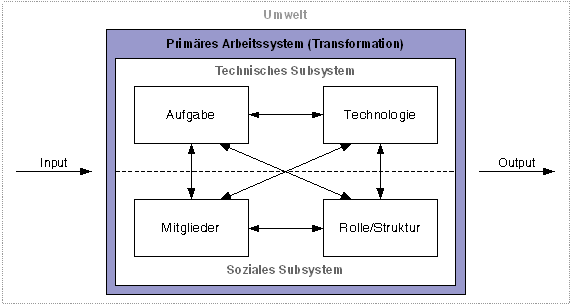
\includegraphics[scale=0.5]{sozio.png}
\end{center}
\end{figure}

Generell besteht ein Sozio-technisches System aus 2 Grundkomponenten. Einer technische Teilkomponente und einer soziale Teilkomponente. Diese haben jeweils weitere Subkomponenten. Das Arbeitssystem besteht aus 2 sozialen Teilkomponenten. Mitgliedern sowie Rollen bzw. Strukturen. Zudem gibt es 2 Technische Teilkomponenten. Eine Technologie, und eine definierte Aufgabe. Alle Teile des Arbeitssystems haben Abhängigkeiten untereinander. Um nun aus einem Input einen Output zu erzeugen, müssen alle Teilkomponenten wechselseitig Interagieren. Fällt eines der Teilkomponenten aus, so ist das gesamte Arbeitssystem nicht mehr lauffähig. Die Technologie bearbeitet und verbessert die Arbeitsprozesse, während die Mitarbeiter ihr Fachwissen und ihre Erfahrung einbringen, um die Systeme zu steuern, zu überwachen und anzupassen. Die Effizienz und Qualität der Produktion hängen sowohl von der technischen Leistungsfähigkeit als auch von der Zusammenarbeit und Interaktion zwischen den Menschen und der Technologie ab. Die Betrachtung von sozio-technischen Systemen ist wichtig, um die Auswirkungen technologischer Veränderungen auf die Arbeitswelt, die Gesellschaft und die Menschen zu verstehen. Es fördert einen ganzheitlichen Ansatz bei der Gestaltung und Implementierung von Technologie, bei dem soziale, organisatorische und technologische Faktoren berücksichtigt werden, um positive Ergebnisse und ein besseres Zusammenwirken von Mensch und Technologie zu erzielen. Insbesondere kann es helfen Problematiken in komplexen Systemen und Prozessen zu verstehen und richtig einzuordnen. Davon ausgehend können nun Lösungen entwickelt werden, die sowohl technische als auch soziale Aspekte miteinbeziehen.  
\newpage
\subsection{Phishing als Sozio-technisches System}
Phishing ist ein sozio-technisches System, das auf die Manipulation von menschlichem Verhalten abzielt, indem es Technologie und soziale Techniken kombiniert. Es basiert auf dem Missbrauch von Vertrauen und der Ausnutzung von Schwachstellen in der menschlichen Natur. Das sozio-technische Phishing-System besteht aus verschiedenen Elementen, darunter die Erstellung gefälschter Websites oder E-Mails, die sich als vertrauenswürdige Quellen ausgeben, um persönliche Daten wie Passwörter oder Kreditkarteninformationen zu stehlen. Es nutzt auch psychologische Techniken, um Dringlichkeit oder Angst zu erzeugen, um Menschen dazu zu bringen, impulsiv zu handeln und persönliche Informationen preiszugeben. Phishing ist ein komplexes Zusammenspiel aus Technologie, sozialem Engineering und menschlichem Verhalten, das es Angreifern ermöglicht, effektiv Informationen zu stehlen und finanziellen Schaden anzurichten. Ein tiefgreifendes Verständnis des sozio-technischen Phishing-Systems ist von entscheidender Bedeutung, um wirksame Schutzmaßnahmen zu entwickeln und die Öffentlichkeit über die Gefahren und Präventionsstrategien aufzuklären.
Betrachtet man Phishing aus dieser Sicht, fällt schnell auf, das bei eine kombination von technischen und sozialen aspekten nutzt. Dies kann wie folgt modeliert werden. 
\section{Angriffslanndschaft}
\section{Systematik von Phishing Prävention}
\section{Technische Lösungsansätze}
\subsection{DNS-Header}
\section{Container}
\bibliographystyle{alpha}
\bibliography{ref.bib}
\end{document}
